\documentclass[10pt,leqno]{amsart}
\usepackage{graphicx}
\baselineskip=16pt

\usepackage{indentfirst,csquotes}
\usepackage{float}
\usepackage{tikz}

\topmargin= .5cm
\textheight= 20cm
\textwidth= 32cc
\baselineskip=16pt

\evensidemargin= .9cm
\oddsidemargin= .9cm

\usepackage{amssymb,amsthm,amsmath}
\usepackage{xcolor,paralist,hyperref,fancyhdr,etoolbox}
\usepackage{listings}

\newtheorem{theorem}{Theorem}[]
\newtheorem{definition}[theorem]{Definition}
\newtheorem{example}[theorem]{Example}
\newtheorem{lemma}[theorem]{Lemma}
\newtheorem{proposition}[theorem]{Proposition}
\newtheorem{corollary}[theorem]{Corollary}
\newtheorem{conjecture}[theorem]{Conjecture}

\hypersetup{ colorlinks=true, linkcolor=black, filecolor=black, urlcolor=black }
\def\proof{\noindent {\it Proof. $\, $}}
\def\endproof{\hfill $\Box$ \vskip 5 pt }
\setcounter{section}{-1}

% Code listing style
\lstset{
  language=C,
  basicstyle=\ttfamily\small,
  keywordstyle=\color{blue}\bfseries,
  commentstyle=\color{gray}\itshape,
  stringstyle=\color{red},
  numbers=none,
  breaklines=true,
  frame=single,
  backgroundcolor=\color{gray!5},
  xleftmargin=1em,
  xrightmargin=1em,
  aboveskip=0.8em,
  belowskip=0.8em,
  columns=fullflexible,
  keepspaces=true,
  showstringspaces=false,
  morekeywords={pragma,omp,parallel,for,single,schedule,static,guided}
}

\begin{document}

\begin{titlepage}
\centering
\vspace*{2cm}

{\LARGE \bfseries C2 High Performance Computing Coursework Report\par}

\vspace{1.5cm}

{\large Baiyuan Chen\par}
\vspace{0.3cm}
{\large CRSID: bc654\par}
\vspace{0.3cm}
{\large bc654@cam.ac.uk\par}

\vspace{1.5cm}

{\large Word Count: 2098\par}

\vspace{1.5cm}

{\large MPhil in Data Intensive Science\par}
\vspace{0.3cm}
{\large University of Cambridge\par}
\vspace{1.5cm}

\vfill
\end{titlepage}

\setcounter{section}{-1}
\section{Introduction}

This report describes the incremental development of an OpenMP-parallelized 
Cholesky factorization routine for symmetric positive-definite matrices. 
All benchmarks were run on the CSD3 
\textbf{icelake} partition (Intel Xeon Platinum 8360Y, 76 cores per node) 
unless otherwise stated. The code is compiled with 
\texttt{gcc -O3 -march=native -funroll-loops -fopenmp}.

\subsection{Project structure}

The repository is organized as follows:
\begin{itemize}
  \item \texttt{src/} --- library source files (\texttt{cholesky\_baseline.c}, 
  \ldots, \texttt{cholesky\_omp3.c}).
  \item \texttt{include/} --- public header \texttt{mphil\_dis\_cholesky.h}.
  \item \texttt{example/} --- example program (\texttt{main.c}) demonstrating 
  usage of the library.
  \item \texttt{test/} --- correctness tests and benchmarking infrastructure.
  \item \texttt{report/} --- this report.
\end{itemize}

\subsection{Testing and correctness verification}

The test suite (\texttt{test/test\_cholesky.c}) verifies correctness via:
\begin{enumerate}
  \item Hand-computed reference cases (the $2\times 2$ and $3\times 3$ 
  examples from the specification).
  \item Frobenius-norm reconstruction error: $\|LL^T - C\|_F / \|C\|_F < 10^{-10}$.
  \item Comparison of $\log|C|$ against LAPACK's \texttt{dpotrf} at 
  $n = 100, 500, 1000$. LAPACK is used \emph{only} in the test harness as a 
  reference; the library itself uses no external libraries beyond OpenMP.
\end{enumerate}
Tests are built and run via \texttt{make IMPL=omp3 test}, which links the 
test binary against \texttt{-llapack -lblas} (available system-wide on CSD3).

\subsection{Benchmarking}

All benchmarks are automated via two scripts:
\begin{itemize}
  \item \texttt{test/run\_bench\_all.sh} --- builds and benchmarks all 
  implementations, writing timing and $\log|C|$ results to 
  \texttt{test/bench\_results.csv}.
  It also runs a thread-scaling sweep of omp3 at thread counts 1, 2, 4, 8, 
  16, 32, 64, writing results to \texttt{test/bench\_scaling.csv}.
  \item \texttt{test/plot\_bench.py} --- reads the CSV files and produces 
  three plots: execution time vs.\ matrix size, accuracy vs.\ LAPACK, and 
  thread scaling. Requires Python~3 with \texttt{matplotlib}.
\end{itemize}
To reproduce all figures:
\begin{verbatim}
  bash test/run_bench_all.sh 64
  python3 test/plot_bench.py
\end{verbatim}

\section{Optimization Strategy}
Baseline and three optimized versions (opt1, opt2, opt3) are developed incrementally.

\subsection{Baseline}

The baseline implementation follows the algorithm provided in the coursework 
specification directly. For each pivot $p = 0, 1, \ldots, n-1$, it performs 
three steps:

\begin{enumerate}
\item \textbf{Diagonal update:} $c_{pp} \leftarrow \sqrt{c_{pp}}$
\item \textbf{Row and column scaling:} $c_{pj} \leftarrow c_{pj}/c_{pp}$ 
and $c_{ip} \leftarrow c_{ip}/c_{pp}$ for all $i, j > p$.
\item \textbf{Rank-1 trailing update:} $c_{ij} \leftarrow c_{ij} - c_{ip}\cdot c_{pj}$ 
for all $i, j > p$.
\end{enumerate}

The trailing update dominates the cost. Since both the inner and outer loops 
of the update iterate over $O(n-p)$ elements, each step is $O((n-p)^2)$, and 
summing over all pivots gives a total complexity of $O(n^3/3)$. In the 
baseline, the inner loops are ordered with $j$ outer and $i$ inner:

\begin{lstlisting}
for (int j = p + 1; j < n; j++)
    for (int i = p + 1; i < n; i++)
        c[i*N + j] -= c[i*N + p] * c[p*N + j];
\end{lstlisting}

This ordering is suboptimal for row-major storage: the inner loop strides 
over \texttt{c[i*N+j]} with stride $N$ (one cache line per iteration), 
causing frequent cache misses.

\subsection{opt1: Loop reordering and micro-optimizations}

Three changes are introduced in opt1:

\noindent\textbf{Loop swap.} The inner loops of the trailing update are 
reordered so that $i$ is outer and $j$ is inner:

\begin{lstlisting}
for (int i = p + 1; i < n; i++) {
    double c_ip = c[i*N + p];      // hoisted invariant
    for (int j = p + 1; j < n; j++)
        c[i*N + j] -= c_ip * c[p*N + j];
}
\end{lstlisting}

Now the inner loop accesses \texttt{c[i*N+j]} and \texttt{c[p*N+j]} with 
stride~1, so consecutive iterations hit the same cache line. For a 64-byte 
cache line holding 8 doubles, this reduces the number of cache line fetches 
by up to $8\times$ compared to the baseline's stride-$N$ access.

\noindent\textbf{Invariant hoisting.} The value \texttt{c[i*N+p]} is 
constant throughout the inner $j$-loop, so it is loaded once into a register 
(\texttt{c\_ip}), avoiding a redundant memory access per inner iteration.

\noindent\textbf{Reciprocal multiply.} The row and column scaling steps 
replace division by \texttt{diag} with multiplication by \texttt{1.0/diag}. 
On modern x86 microarchitectures, \texttt{MULSD} has a throughput of 1 cycle 
vs.\ 4--6 cycles for \texttt{DIVSD}, giving a $4$--$6\times$ speedup on this 
operation. The cost of computing the reciprocal once ($\sim$20 cycles) is 
amortized over $O(n)$ multiplications.

\subsection{opt2: Batched rank-1 updates (blocked panel factorization)}
 
\noindent In opt1, each pivot $p$ applies a rank-1 update to the trailing
submatrix of size $(n-p-1)^2$. For large $n$, this submatrix far exceeds
cache capacity, so every rank-1 update streams the entire trailing matrix
from main memory. Over $n$ pivots, the total memory traffic is $O(n^3)$
doubles.
 
The fix is to \emph{delay} the trailing update. opt2 groups
$N_B = 64$ consecutive pivots into a \emph{panel} and applies all their
updates in one pass---reducing memory traffic by a factor of $\sim N_B$.
Each panel is processed in three phases (illustrated in
Figure~\ref{fig:phases} for $n=12$, $N_B=4$):
 
\noindent\textbf{Phase A} (panel factorization): run the unblocked opt1
algorithm on just the $N_B$ columns of the panel, factoring the diagonal
block and scaling the column panel below it. The $j$-loop stays within
the panel boundary and the trailing matrix is not touched.
 
\noindent\textbf{Phase B} (upper row solve): rows $pp$ through
$pp{+}N_B{-}1$ still have stale values to the right of the panel. For
each such row, contributions from earlier panel rows are subtracted and
the result is scaled by the diagonal (the same treatment opt1 would
have applied). This is $O(N_B^2 \cdot m)$, small compared to Phase~C.
 
\noindent\textbf{Phase C} (trailing update): apply a single rank-$N_B$
update, combining all 64 pivots into one pass:
 
\begin{lstlisting}
for (int i = pp + pb; i < n; i++) {
    for (int k = pp; k < pp + pb; k++) {
        double c_ik = c[i*N + k];
        for (int j = pp + pb; j < n; j++)
            c[i*N + j] -= c_ik * c[k*N + j];
    }
}
\end{lstlisting}
 
When the CPU loads row $i$ into cache, the $k$-loop runs 64 times before
moving on. The panel data ($N_B \times 8 = 512$ bytes) fits in L1, so the
trailing matrix passes through memory $n/N_B$ times instead of $n$ times.
$N_B = 64$ is chosen to fit within the 48\,KB L1 cache of the Icelake core.
 
\begin{figure}[H]
\centering
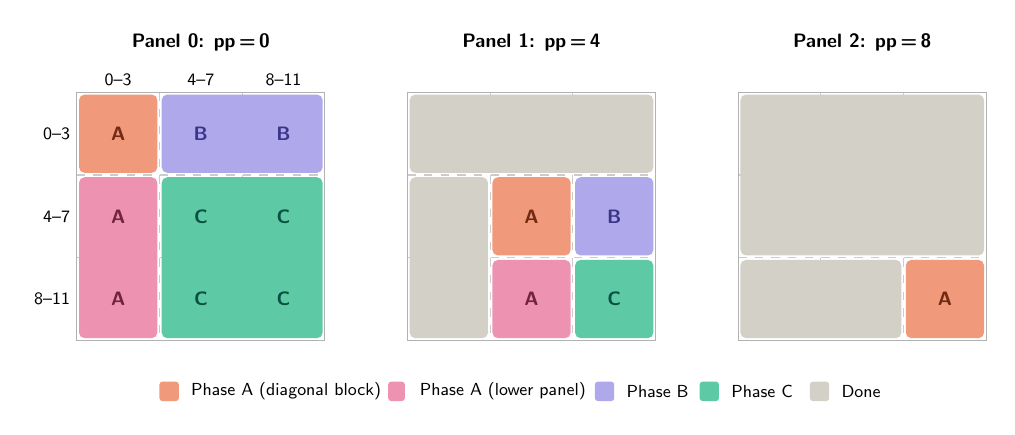
\begin{tikzpicture}[scale=0.7, transform shape,
    block/.style={minimum size=1.5cm, rounded corners=2pt, 
                  font=\sffamily\bfseries\large, text opacity=1},
    label/.style={font=\small\sffamily},
]
 
% Colors
\definecolor{phA}{HTML}{F0997B}
\definecolor{phAl}{HTML}{ED93B1}
\definecolor{phB}{HTML}{AFA9EC}
\definecolor{phC}{HTML}{5DCAA5}
\definecolor{done}{HTML}{D3D1C7}
\definecolor{tA}{HTML}{712B13}
\definecolor{tAl}{HTML}{72243E}
\definecolor{tB}{HTML}{3C3489}
\definecolor{tC}{HTML}{085041}
 
\newcommand{\drawgrid}[1]{%
  \draw[gray!40, dashed, thin] (#1+1.5,0) -- (#1+1.5,-4.5);
  \draw[gray!40, dashed, thin] (#1+3.0,0) -- (#1+3.0,-4.5);
  \draw[gray!40, dashed, thin] (#1,  -1.5) -- (#1+4.5,-1.5);
  \draw[gray!40, dashed, thin] (#1,  -3.0) -- (#1+4.5,-3.0);
  \draw[gray!60] (#1,0) rectangle (#1+4.5,-4.5);
}
 
\newcommand{\drawlabels}[1]{%
  \node[label, above] at (#1+0.75, 0) {0--3};
  \node[label, above] at (#1+2.25, 0) {4--7};
  \node[label, above] at (#1+3.75, 0) {8--11};
  \node[label, left]  at (#1, -0.75)  {0--3};
  \node[label, left]  at (#1, -2.25)  {4--7};
  \node[label, left]  at (#1, -3.75)  {8--11};
}
 
% === Panel 0: pp=0 ===
\def\px{0}
\node[font=\sffamily\bfseries] at (\px+2.25, 0.9) {Panel 0: pp\,=\,0};
\drawgrid{\px}
\drawlabels{\px}
 
\fill[phA,  rounded corners=2pt] (\px+0.04,-0.04) rectangle (\px+1.46,-1.46);
\fill[phAl, rounded corners=2pt] (\px+0.04,-1.54) rectangle (\px+1.46,-4.46);
\fill[phB,  rounded corners=2pt] (\px+1.54,-0.04) rectangle (\px+4.46,-1.46);
\fill[phC,  rounded corners=2pt] (\px+1.54,-1.54) rectangle (\px+4.46,-4.46);
 
\node[tA]  at (\px+0.75, -0.75) {\textsf{\textbf{A}}};
\node[tAl] at (\px+0.75, -2.25) {\textsf{\textbf{A}}};
\node[tAl] at (\px+0.75, -3.75) {\textsf{\textbf{A}}};
\node[tB]  at (\px+2.25, -0.75) {\textsf{\textbf{B}}};
\node[tB]  at (\px+3.75, -0.75) {\textsf{\textbf{B}}};
\node[tC]  at (\px+2.25, -2.25) {\textsf{\textbf{C}}};
\node[tC]  at (\px+3.75, -2.25) {\textsf{\textbf{C}}};
\node[tC]  at (\px+2.25, -3.75) {\textsf{\textbf{C}}};
\node[tC]  at (\px+3.75, -3.75) {\textsf{\textbf{C}}};
 
% === Panel 1: pp=4 ===
\def\px{6}
\node[font=\sffamily\bfseries] at (\px+2.25, 0.9) {Panel 1: pp\,=\,4};
\drawgrid{\px}
 
\fill[done, rounded corners=2pt] (\px+0.04,-0.04) rectangle (\px+4.46,-1.46);
\fill[done, rounded corners=2pt] (\px+0.04,-1.54) rectangle (\px+1.46,-4.46);
\fill[phA,  rounded corners=2pt] (\px+1.54,-1.54) rectangle (\px+2.96,-2.96);
\fill[phAl, rounded corners=2pt] (\px+1.54,-3.04) rectangle (\px+2.96,-4.46);
\fill[phB,  rounded corners=2pt] (\px+3.04,-1.54) rectangle (\px+4.46,-2.96);
\fill[phC,  rounded corners=2pt] (\px+3.04,-3.04) rectangle (\px+4.46,-4.46);
 
\node[tA]  at (\px+2.25, -2.25) {\textsf{\textbf{A}}};
\node[tAl] at (\px+2.25, -3.75) {\textsf{\textbf{A}}};
\node[tB]  at (\px+3.75, -2.25) {\textsf{\textbf{B}}};
\node[tC]  at (\px+3.75, -3.75) {\textsf{\textbf{C}}};
 
% === Panel 2: pp=8 ===
\def\px{12}
\node[font=\sffamily\bfseries] at (\px+2.25, 0.9) {Panel 2: pp\,=\,8};
\drawgrid{\px}
 
\fill[done, rounded corners=2pt] (\px+0.04,-0.04) rectangle (\px+4.46,-2.96);
\fill[done, rounded corners=2pt] (\px+0.04,-3.04) rectangle (\px+2.96,-4.46);
\fill[phA,  rounded corners=2pt] (\px+3.04,-3.04) rectangle (\px+4.46,-4.46);
 
\node[tA] at (\px+3.75, -3.75) {\textsf{\textbf{A}}};
 
% === Legend ===
\def\ly{-5.6}
\fill[phA,  rounded corners=1pt] (1.5,\ly) rectangle (1.85,\ly+0.35);
\node[anchor=west, font=\small\sffamily] at (1.95,\ly+0.175) {Phase A (diagonal block)};
\fill[phAl, rounded corners=1pt] (5.65,\ly) rectangle (5.95,\ly+0.35);
\node[anchor=west, font=\small\sffamily] at (6.1,\ly+0.175) {Phase A (lower panel)};
\fill[phB,  rounded corners=1pt] (9.4,\ly) rectangle (9.75,\ly+0.35);
\node[anchor=west, font=\small\sffamily] at (9.85,\ly+0.175) {Phase B};
\fill[phC,  rounded corners=1pt] (11.3,\ly) rectangle (11.65,\ly+0.35);
\node[anchor=west, font=\small\sffamily] at (11.75,\ly+0.175) {Phase C};
\fill[done, rounded corners=1pt] (13.3,\ly) rectangle (13.65,\ly+0.35);
\node[anchor=west, font=\small\sffamily] at (13.75,\ly+0.175) {Done};
\end{tikzpicture}
\caption{Blocked Cholesky phase map for $n=12$, $N_B=4$. Phase~C
(trailing update) dominates the cost and shrinks each iteration. By the
final panel only Phase~A remains.}
\label{fig:phases}
\end{figure}

\subsection{opt3: Lower-triangle-only trailing update}

In opt2, Phase~C updates the \emph{full} trailing submatrix, but since $C$
is symmetric, only the lower triangle is actually needed. The upper triangle
is just a copy of the lower, and Phase~B of the next panel will overwrite it
anyway. This means roughly half the FLOPs in Phase~C are wasted.
 
opt3 makes three changes to exploit this:
 
\textit{(i) Phase~C restricted to the lower triangle.} The inner $j$-loop bound changes from \texttt{j < n} to \texttt{j <= i}:
 
\begin{lstlisting}
for (int i = pp + pb; i < n; i++)
    for (int k = pp; k < pp + pb; k++) {
        double c_ik = c[i*N + k];
        for (int j = pp + pb; j <= i; j++)
            c[i*N + j] -= c_ik * c[k*N + j];
    }
\end{lstlisting}
 
The total FLOP count for Phase~C drops from $m^2 \cdot N_B$ to $\tfrac{1}{2}m^2 \cdot N_B$, nearly doubling throughput for large $m$.
 
\textit{(ii) Phase~B replaced by transpose copy.} Since Phase~C now only writes the lower triangle, the upper-triangular entries $c_{kj}$ for $k < pp + N_B \leq j$ needed by the next Phase~C are simply $L^T_{kj} = L_{jk} = c_{jk}$. The entire triangular solve is replaced by a copy:
 
\begin{lstlisting}
for (int k = pp; k < pp + pb; k++)
    for (int j = pp + pb; j < n; j++)
        c[k*N + j] = c[j*N + k];
\end{lstlisting}
 
This replaces $O(N_B^2 \cdot m)$ FLOPs with $O(N_B \cdot m)$ memory copies, eliminating Phase~B as a cost centre entirely.
 
\textit{(iii) Mirror step.} Before each Phase~A, the lower triangle of the current $N_B \times N_B$ diagonal block is copied to its upper triangle, since the previous Phase~C only wrote the lower entries:
 
\begin{lstlisting}
if (pp > 0)
    for (int i = pp + 1; i < pp + pb; i++)
        for (int j = pp; j < i; j++)
            c[j*N + i] = c[i*N + j];
\end{lstlisting}
 
This is $O(N_B^2)$ per panel --- negligible compared to Phase~C.

\section{Parallelization Strategy}

\subsection{omp1: Basic OpenMP parallelization}

omp1 adds OpenMP directives to the opt1 algorithm. A single persistent 
parallel region wraps the entire pivot loop, avoiding repeated fork/join 
overhead (which can cost $\sim$10\,$\mu$s per fork on modern systems):

\begin{lstlisting}
#pragma omp parallel
{
    for (int p = 0; p < n; p++) {
        #pragma omp single
        {   // diagonal update: single scalar op
            double diag = sqrt(c[p*N + p]);
            c[p*N + p] = diag;
            inv_diag = 1.0 / diag;
        }   // implicit barrier

        #pragma omp for schedule(static)
        for (int j = p + 1; j < n; j++)
            c[p*N + j] *= inv_diag;

        #pragma omp for schedule(static)
        for (int i = p + 1; i < n; i++)
            c[i*N + p] *= inv_diag;

        #pragma omp for schedule(static)
        for (int i = p + 1; i < n; i++) {
            double c_ip = c[i*N + p];
            for (int j = p + 1; j < n; j++)
                c[i*N + j] -= c_ip * c[p*N + j];
        }
    }
}
\end{lstlisting}

The diagonal update is performed by a single thread via 
\texttt{\#pragma omp single}; the implicit barrier after the 
\texttt{single} block ensures that all threads observe the updated 
\texttt{inv\_diag} before proceeding. The row scaling, column scaling, and 
trailing update are parallelized over their respective loop indices. Each 
iteration is independent (no write conflicts), so no atomic operations or 
critical sections are required. Static scheduling is used because all rows 
have equal work ($n-p-1$ multiplications).

\subsection{omp2: Blocked + parallel}

omp2 combines the blocking strategy of opt2 with OpenMP parallelization. The 
same persistent parallel region encloses the outer panel loop.

\noindent\textbf{Phase A.} Within the panel, each pivot $k$ depends on the 
previous one (the rank-1 update must complete before the next diagonal is 
computed), so the $k$-loop is inherently sequential. However, the column 
scaling below the panel and the rank-1 update on the lower panel are 
parallelized across threads via \texttt{\#pragma omp for}:

\begin{lstlisting}
// Scale column below pk --- parallelized
#pragma omp for schedule(static)
for (int i = pk + 1; i < n; i++)
    c[i*N + pk] *= inv;

// Rank-1 update on lower panel --- parallelized
#pragma omp for schedule(static)
for (int i = pp + pb; i < n; i++) {
    double c_ip = c[i*N + pk];
    for (int j = pk + 1; j < pp + pb; j++)
        c[i*N + j] -= c_ip * c[pk*N + j];
}
\end{lstlisting}

The small intra-block operations (row scaling within the panel, rank-1 
update within the diagonal block) are executed by a single thread via 
\texttt{\#pragma omp single}, since the overhead of distributing $O(N_B^2)$ 
work across threads would exceed the computation cost.

\noindent\textbf{Phase B.} The triangular solve is $O(N_B^2 \cdot m)$, which 
is small relative to Phase~C's $O(m^2 \cdot N_B)$. It is executed by a 
single thread inside a \texttt{\#pragma omp single} block.

\noindent\textbf{Phase C.} The dominant trailing update is parallelized by 
distributing rows across threads:

\begin{lstlisting}
#pragma omp for schedule(static)
for (int i = pp + pb; i < n; i++) {
    for (int k = pp; k < pp + pb; k++) {
        double c_ik = c[i*N + k];
        for (int j = pp + pb; j < n; j++)
            c[i*N + j] -= c_ik * c[k*N + j];
    }
}
\end{lstlisting}

Each row $i$ is fully independent (no shared write targets), so no 
synchronization is needed within Phase~C. Static scheduling is appropriate 
here because every row performs the same amount of work: $N_B \times m$ 
multiply-subtract operations.

\subsection{omp3: Guided scheduling for triangular workload}

omp3 builds on omp2 but incorporates the lower-triangle-only optimization 
from opt3. This introduces a key scheduling challenge.

In Phase~C with the lower-triangle restriction, row $i$ performs work 
proportional to $(i - pp - N_B + 1)$ rather than a constant $m$. Concretely, 
with $T$ threads and static scheduling, each thread receives a contiguous 
chunk of $m/T$ consecutive rows. The thread assigned to the \emph{last} 
chunk (rows with the largest indices) does:
\begin{equation}
W_{\text{last}} = \sum_{i=m - m/T}^{m-1} i \;\approx\; \frac{m^2}{2T}\left(2 - \frac{1}{T}\right)
\end{equation}
while the ideal per-thread share is:
\begin{equation}
W_{\text{ideal}} = \frac{1}{T}\sum_{i=0}^{m-1} i \;=\; \frac{m^2}{2T}
\end{equation}
For $T = 4$, the last thread does $\approx 44\%$ of the total work (vs.\ the 
ideal 25\%), leaving 3 threads idle for nearly half the phase.

To address this imbalance, \texttt{schedule(static)} is replaced with 
\texttt{schedule(guided)} in the Phase~C loop is effective:

\begin{lstlisting}
#pragma omp for schedule(guided)
for (int i = pp + pb; i < n; i++) {
    for (int k = pp; k < pp + pb; k++) {
        double c_ik = c[i*N + k];
        for (int j = pp + pb; j <= i; j++)
            c[i*N + j] -= c_ik * c[k*N + j];
    }
}
\end{lstlisting}

Guided scheduling assigns chunks of size $\max(\lceil R/T \rceil, 1)$
where $R$ is the number of remaining iterations and $T$ is the number of
threads. This produces geometrically decreasing chunk sizes: the first
chunks are large and cover the early, light rows (low $i$), while the
last chunks are small and cover the late, heavy rows (high $i$). A thread
that receives a large chunk of light rows ends up doing roughly the same
total work as a thread that receives a small chunk of heavy rows, naturally
balancing the triangular workload.

Moreover, the transpose copy that replaces the triangular solve is also 
parallelized:

\begin{lstlisting}
#pragma omp for schedule(static)
for (int k = pp; k < pp + pb; k++)
    for (int j = pp + pb; j < n; j++)
        c[k*N + j] = c[j*N + k];
\end{lstlisting}

Each row $k$ writes to disjoint memory locations, so no synchronization is 
needed. Static scheduling is used here because all rows perform the same 
amount of work ($m$ copies each).

\section{Performance Results}

\subsection{Execution time vs.\ matrix size}

Figure~\ref{fig:time} shows the execution time across all implementations 
for matrix sizes $n = 100$ to $10{,}000$.

\begin{figure}[htbp]
\centering
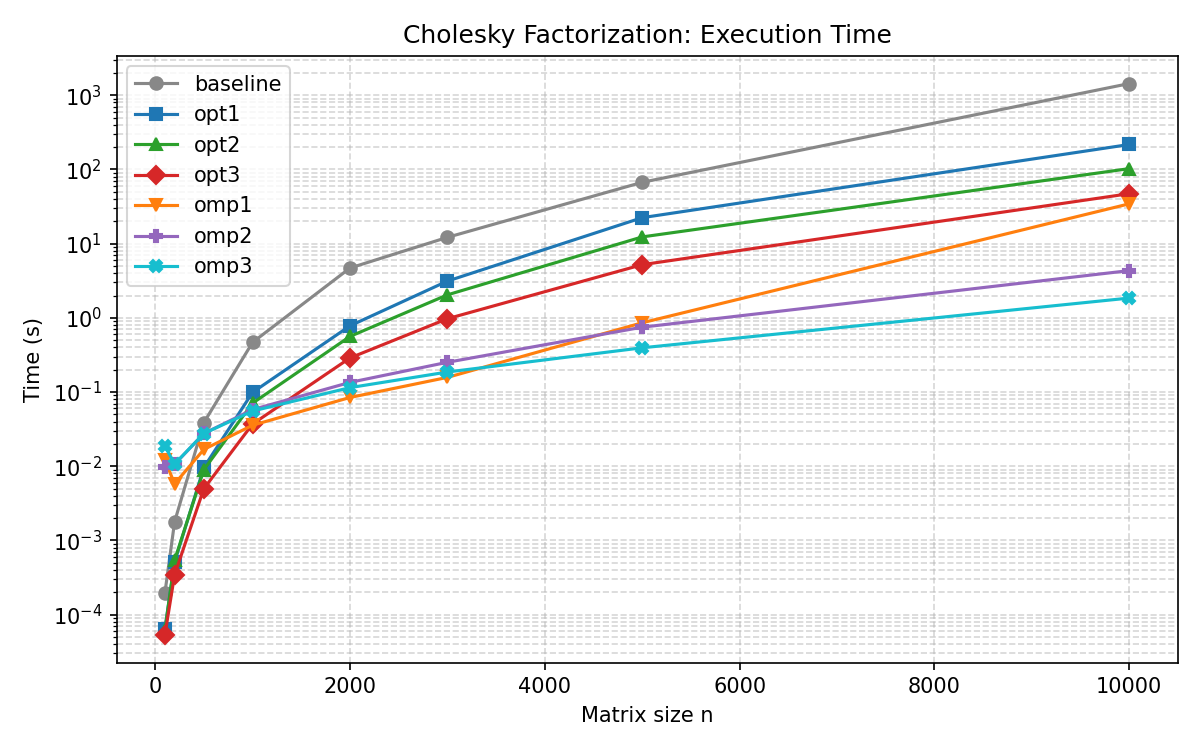
\includegraphics[width=0.7\textwidth]{../test/bench_time.png}
\caption{Execution time vs.\ matrix size for all implementations 
(OMP\_NUM\_THREADS=64, icelake partition).}
\label{fig:time}
\end{figure}

The single-threaded optimizations each build on the last: at $n{=}1000$,
opt1 is roughly $5\times$ faster than the baseline (0.099\,s vs.\ 0.467\,s)
from better cache access patterns alone, opt2 brings this down to 0.071\,s
with blocking, and opt3 reaches 0.037\,s by halving the trailing-update work.

Parallelism only pays off once the matrix is large enough. At $n{=}500$,
opt3 (0.005\,s) actually beats omp3 (0.028\,s) by over $5\times$---the
matrix is small enough to fit in cache, so the overhead of synchronizing
64 threads (barriers, single-region handoffs, cache-coherence traffic)
outweighs any benefit from splitting the work. Beyond $n \approx 1000$ the
cubic growth in computation begins to dominate these fixed costs, and by
$n{=}10{,}000$ omp3 (1.85\,s) is ${\sim}25\times$ faster than opt3
(47.2\,s).

Among the parallel variants, the gap between omp2 and omp3 grows with
matrix size (4.33\,s vs.\ 1.85\,s at $n{=}10{,}000$): the larger the
matrix, the worse the triangular load imbalance becomes, and the more
guided scheduling and the lower-triangle optimization help.

\subsection{Accuracy vs.\ LAPACK reference}

Figure~\ref{fig:acc} shows the relative error in $\log|C|$ compared to 
LAPACK's \texttt{dpotrf}. All implementations achieve machine-precision 
accuracy ($\sim 10^{-15}$).

\begin{figure}[htbp]
\centering
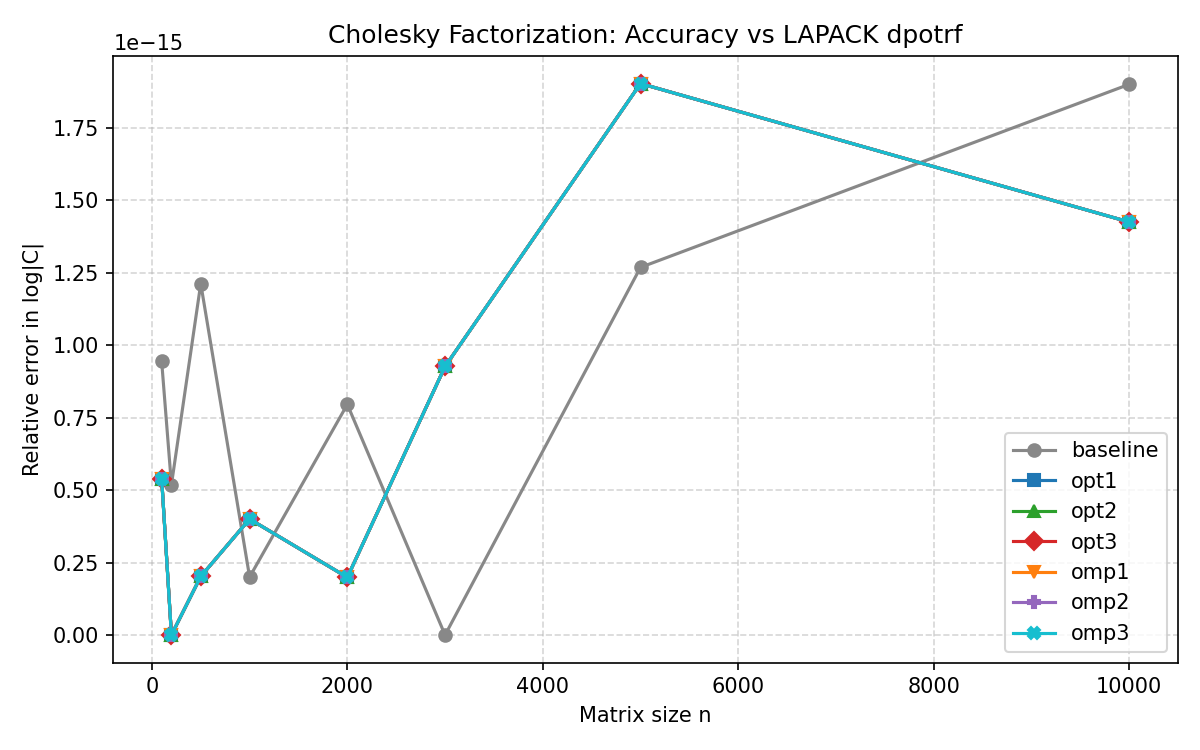
\includegraphics[width=0.7\textwidth]{../test/bench_accuracy.png}
\caption{Relative error in $\log|C|$ vs.\ LAPACK \texttt{dpotrf} reference.}
\label{fig:acc}
\end{figure}

\subsection{Thread scaling}

Figure~\ref{fig:scaling} shows how omp3 scales with thread count for
several matrix sizes.

\begin{figure}[htbp]
\centering
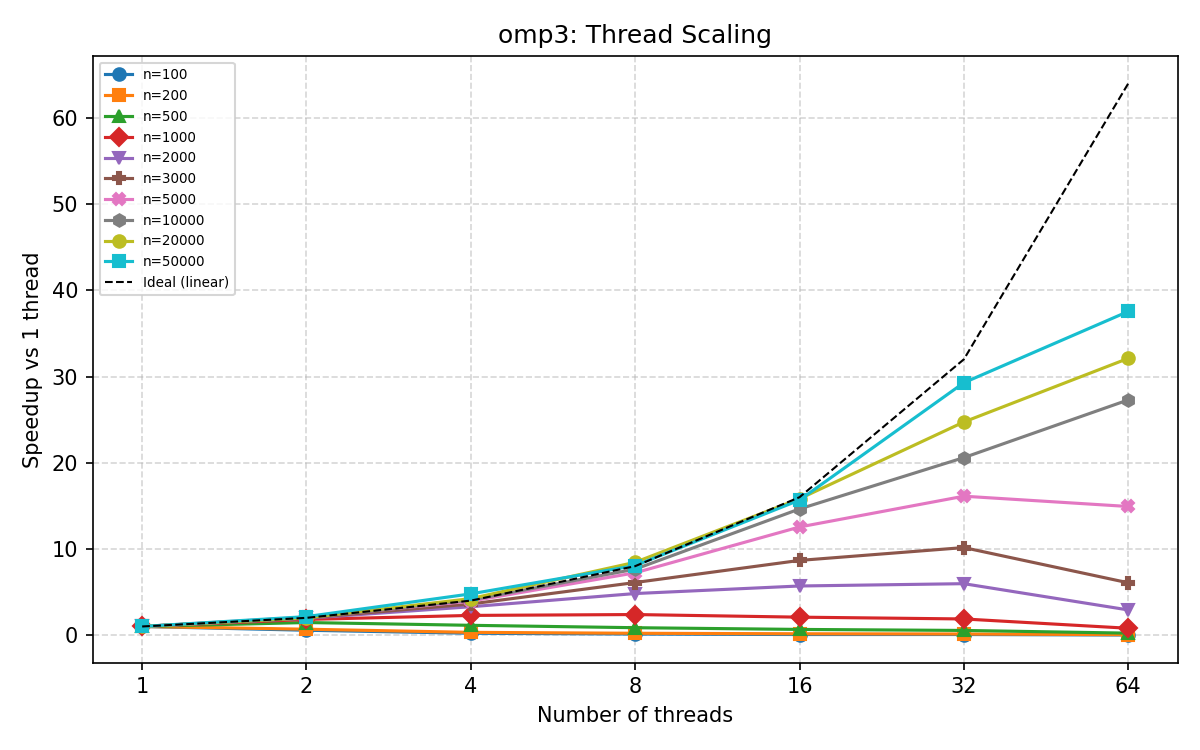
\includegraphics[width=0.7\textwidth]{../test/bench_scaling.png}
\caption{omp3 thread scaling on icelake. Each line represents a fixed
matrix size.}
\label{fig:scaling}
\end{figure}

For small matrices, adding threads makes things worse. At $n{=}100$,
64 threads is over $100\times$ slower than one thread (0.019\,s vs.\
0.0002\,s), because the actual computation is tiny compared to the cost
of barrier synchronization and thread management. The matrix fits in
cache, so there is almost nothing to parallelise.

As $n$ grows and Phase~C begins to dominate the runtime, scaling improves
steadily. At $n{=}10{,}000$, 64 threads gives a $27\times$ speedup; at
$n{=}20{,}000$ this rises to $32\times$; and at $n{=}50{,}000$ it
reaches $37.5\times$, continuing the trend toward the ideal $64\times$ line. 
The gap that remains comes from the serial panel factorisation (Phase~A), 
memory bandwidth saturation across 76 cores sharing the same memory 
controllers, and NUMA effects on the dual-socket node. Still, the trend is 
clear: the larger the matrix, the closer the scaling gets to linear.

\section{Tagged Commits}

Table~\ref{tab:tags} lists the tagged commits corresponding to each 
significant version of the code.

\begin{table}[H]
\centering
\begin{tabular}{l l l}
\hline
\textbf{Tag} & \textbf{Commit} & \textbf{Description} \\
\hline
\texttt{baseline-implementation+test-script} & \texttt{e2dd2639} & Baseline implementation with tests \\
\texttt{single-threaded-opt1-loop-swap} & \texttt{806694b0} & opt1: loop reordering for cache locality \\
\texttt{omp1-loop-swap} & \texttt{ba1f3ea8} & omp1: first parallel version \\
\texttt{opt2/omp2} & \texttt{97adb319} & Blocked updates, reduced memory traffic \\
\texttt{opt3/omp3} & \texttt{4fa64c34} & Lower-triangle update, guided scheduling \\
\hline
\end{tabular}
\caption{Tagged commits in the Git history.}
\label{tab:tags}
\end{table}

\section{Conclusion}

The final implementation (omp3) combines loop reordering for cache locality,
blocked panel factorization to reduce memory traffic by $\sim 64\times$, and
lower-triangle-only updates to halve Phase~C FLOPs, with guided OpenMP
scheduling to balance the triangular workload. All implementations match
LAPACK's \texttt{dpotrf} to machine precision.

\section*{Use of generative AI}
Claude (Anthropic) was used to assist with code development and
report writing. All outputs were reviewed and tested by the author,
who takes full responsibility for the final submission.

% \begin{thebibliography}{99}
% \bibitem{1} ***
% \end{thebibliography}

\end{document}